\documentclass[11pt,]{article}
\usepackage[left=1in,top=1in,right=1in,bottom=1in]{geometry}
\newcommand*{\authorfont}{\fontfamily{phv}\selectfont}
\usepackage[]{mathpazo}


  \usepackage[T1]{fontenc}
  \usepackage[utf8]{inputenc}



\usepackage{abstract}
\renewcommand{\abstractname}{}    % clear the title
\renewcommand{\absnamepos}{empty} % originally center

\renewenvironment{abstract}
 {{%
    \setlength{\leftmargin}{0mm}
    \setlength{\rightmargin}{\leftmargin}%
  }%
  \relax}
 {\endlist}

\makeatletter
\def\@maketitle{%
  \newpage
%  \null
%  \vskip 2em%
%  \begin{center}%
  \let \footnote \thanks
    {\fontsize{18}{20}\selectfont\raggedright  \setlength{\parindent}{0pt} \@title \par}%
}
%\fi
\makeatother




\setcounter{secnumdepth}{3}

\usepackage{longtable,booktabs}

\usepackage{graphicx,grffile}
\makeatletter
\def\maxwidth{\ifdim\Gin@nat@width>\linewidth\linewidth\else\Gin@nat@width\fi}
\def\maxheight{\ifdim\Gin@nat@height>\textheight\textheight\else\Gin@nat@height\fi}
\makeatother
% Scale images if necessary, so that they will not overflow the page
% margins by default, and it is still possible to overwrite the defaults
% using explicit options in \includegraphics[width, height, ...]{}
\setkeys{Gin}{width=\maxwidth,height=\maxheight,keepaspectratio}

\title{Mis hormigas\\
Subtítulo\\
Subtítulo  }



\author{\Large Emma M. Diloné Ricardo\vspace{0.05in} \newline\normalsize\emph{Estudiante, Universidad Autónoma de Santo Domingo (UASD)}  }


\date{}

\usepackage{titlesec}

\titleformat*{\section}{\normalsize\bfseries}
\titleformat*{\subsection}{\normalsize\itshape}
\titleformat*{\subsubsection}{\normalsize\itshape}
\titleformat*{\paragraph}{\normalsize\itshape}
\titleformat*{\subparagraph}{\normalsize\itshape}

\titlespacing{\section}
{0pt}{36pt}{0pt}
\titlespacing{\subsection}
{0pt}{36pt}{0pt}
\titlespacing{\subsubsection}
{0pt}{36pt}{0pt}





\newtheorem{hypothesis}{Hypothesis}
\usepackage{setspace}

\makeatletter
\@ifpackageloaded{hyperref}{}{%
\ifxetex
  \PassOptionsToPackage{hyphens}{url}\usepackage[setpagesize=false, % page size defined by xetex
              unicode=false, % unicode breaks when used with xetex
              xetex]{hyperref}
\else
  \PassOptionsToPackage{hyphens}{url}\usepackage[unicode=true]{hyperref}
\fi
}

\@ifpackageloaded{color}{
    \PassOptionsToPackage{usenames,dvipsnames}{color}
}{%
    \usepackage[usenames,dvipsnames]{color}
}
\makeatother
\hypersetup{breaklinks=true,
            bookmarks=true,
            pdfauthor={Emma M. Diloné Ricardo (Estudiante, Universidad Autónoma de Santo Domingo (UASD))},
             pdfkeywords = {palabra clave 1, palabra clave 2},  
            pdftitle={Mis hormigas\\
Subtítulo\\
Subtítulo},
            colorlinks=true,
            citecolor=blue,
            urlcolor=blue,
            linkcolor=magenta,
            pdfborder={0 0 0}}
\urlstyle{same}  % don't use monospace font for urls

% set default figure placement to htbp
\makeatletter
\def\fps@figure{htbp}
\makeatother

\usepackage{pdflscape} \newcommand{\blandscape}{\begin{landscape}}
\newcommand{\elandscape}{\end{landscape}}


% add tightlist ----------
\providecommand{\tightlist}{%
\setlength{\itemsep}{0pt}\setlength{\parskip}{0pt}}

\begin{document}
	
% \pagenumbering{arabic}% resets `page` counter to 1 
%
% \maketitle

{% \usefont{T1}{pnc}{m}{n}
\setlength{\parindent}{0pt}
\thispagestyle{plain}
{\fontsize{18}{20}\selectfont\raggedright 
\maketitle  % title \par  

}

{
   \vskip 13.5pt\relax \normalsize\fontsize{11}{12} 
\textbf{\authorfont Emma M. Diloné Ricardo} \hskip 15pt \emph{\small Estudiante, Universidad Autónoma de Santo Domingo (UASD)}   

}

}








\begin{abstract}

    \hbox{\vrule height .2pt width 39.14pc}

    \vskip 8.5pt % \small 

\noindent Mi resumen


\vskip 8.5pt \noindent \emph{Keywords}: palabra clave 1, palabra clave 2 \par

    \hbox{\vrule height .2pt width 39.14pc}



\end{abstract}


\vskip 6.5pt


\noindent  \section{Introducción}\label{introducciuxf3n}

Localización

las hormigas

Las hormigas pertenecen a una sola familia que es la Formicidae, dentro
de la superfamilia Vespoidea (RES (1993)). Forman parte de un grupo de
himenópteros sociales muy diversos, tanto taxonómica como funcionalmente
(Fernández (2001)). Las hormigas, dentro del grupo de los insectos, se
considera como uno de los grupos más evolucionados por el nivel social y
por el grado de especialización y dependencia que estas pueden alcanzar
(REYES (n.d.)).

Distribución de las hormigas

Las hormigas representan una de las familias dominantes en cualquier
ecosistema (REYES (n.d.)).

Hormigas en la isla

En la isla La Hispaniola se conocen 43 géneros y 147 especies y
subespecies de hormigas (\emph{Ants of hispaniola}, n.d.).

Hormigas en el campus de la UASD

No se tiene una publicación que identifique las especies de hormigas que
se encuentran dentro del campus.

El objeto general y especificos.

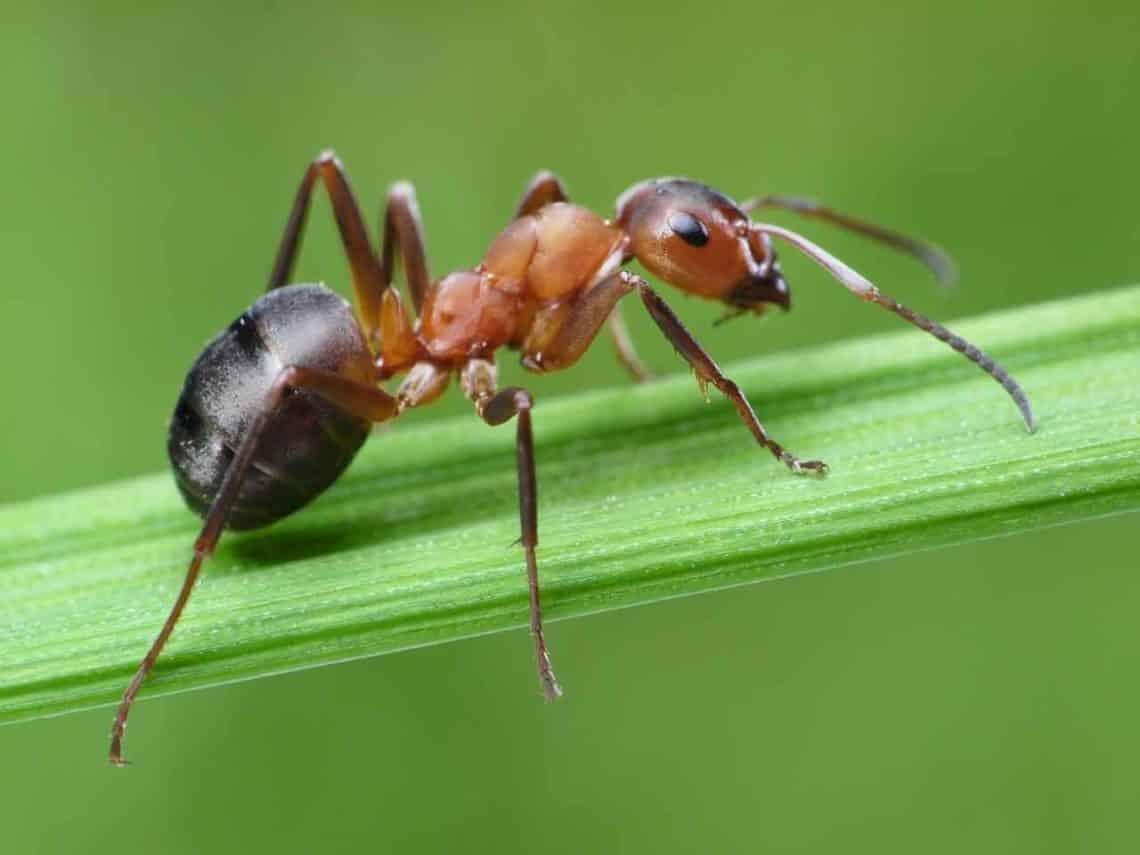
\includegraphics{Hormiga-1.jpg} \# Metodología

\ldots

\section{Resultados}\label{resultados}

tablas y gráficos

\begin{longtable}[]{@{}cccccc@{}}
\toprule
hola & adios & 1 & 2 & 3 & 4\tabularnewline
\midrule
\endhead
& & & & &\tabularnewline
& & & & &\tabularnewline
& & & & &\tabularnewline
\bottomrule
\end{longtable}

\section{Discusión}\label{discusiuxf3n}

conclusión

\section{Agradecimientos}\label{agradecimientos}

\section{Información de soporte}\label{informaciuxf3n-de-soporte}

\ldots

\section{\texorpdfstring{\emph{Script}
reproducible}{Script reproducible}}\label{script-reproducible}

\ldots

\section*{Referencias}\label{referencias}
\addcontentsline{toc}{section}{Referencias}

\hypertarget{refs}{}
\hypertarget{ref-Antwiki}{}
\emph{Ants of hispaniola}. (n.d.).
\url{http://www.antwiki.org/wiki/Ants_of_Hispaniola}.

\hypertarget{ref-fernandez2001hormigas}{}
Fernández, P. R. (2001). Las hormigas del suelo en méxico: Diversidad,
distribución e importancia (hymenoptera: Formicidae). \emph{Acta
Zoológica Mexicana (Nueva Serie)}, (Es1), 189--238.

\hypertarget{ref-res1993phylogeny}{}
RES, J. (1993). Phylogeny of aculeata: Chrysidoidea and vespoidea
(hymenoptera). \emph{J. Hym. Res}, \emph{2}(1), 227--304.

\hypertarget{ref-reyeshormigas}{}
REYES, J. L. (n.d.). Hormigas sinantrópicas en santiago de cuba
(hymenoptera: Formicidae). \emph{COCUYO}, 44.




\newpage
\singlespacing 
\end{document}
